\documentclass[10pt,twocolumn]{article}
\usepackage[margin=0.8in]{geometry}
\usepackage{graphicx,booktabs,amsmath,hyperref,caption}
\usepackage[T1]{fontenc}
\captionsetup{font=small}
\graphicspath{{figures/}}
\newcommand{\todo}[1]{\textbf{[#1]}}

\title{How Much Does a Zero-Resource Hallucination Detector Beat Trivial Heuristics? Sample Budget, Controls and Threshold Robustness for SelfCheck-NGram on WikiBio-GPT-3}
\author{Kushagra Agrawal (MHM2026009)\\ M.Tech.\ Information Technology (Human Machine Interaction)\\ Course: AI Tools for Research --- Lab 02 implementation paper}
\date{}

\begin{document}
\maketitle

\begin{abstract}
My earlier literature review on hallucination types in large language models (topic T20) listed calibrated abstention as an open need; any abstention rule needs a detection signal. This paper asks how good a cheap, zero-resource, sampling-based detector is. I evaluate the unigram variant of SelfCheck-NGram on 1,908 human-labelled sentences from 238 GPT-3 biographies, varying the number of sampled passages ($k=5,10,20$), using five random subset seeds, biography-level bootstrap confidence intervals, and three trivial controls (sentence position, sentence length, random). AUROC rises from 0.589 ($k=5$) to 0.655 ($k=20$); the paired improvement is $+0.066$ (95\% CI 0.053--0.079). However, at $k=5$ the detector is statistically indistinguishable from the sentence-position control (AUROC difference $+0.007$, CI $-0.036$ to $0.047$), and at $k=20$ the margin over that control is only $+0.073$ (CI 0.033--0.115). Average precision looks high (0.815) mainly because 73\% of sentences are inaccurate. At the best single threshold, about half of accurate sentences are flagged. I conclude that the unigram detector carries a real but weak signal that is easy to over-read; I did not test stronger detectors. The protocol was fixed retrospectively, and all results come from the code and CSV files in the accompanying repository.
\end{abstract}

\section{Introduction}
Hallucination in generated text is a central concern for research use of language models, and my first paper (a literature review, topic T20) catalogued its types and open problems, among them calibrated abstention \todo{TO VERIFY: cite review section/page}. Abstaining or flagging a sentence requires a score that separates accurate from inaccurate content. SelfCheckGPT \cite{manakul2023selfcheckgpt} proposes such a score without external knowledge: sample several answers from the same model and treat inconsistency with the samples as a sign of hallucination.

This study is a controlled comparison, not a new method. It asks:
\begin{itemize}\setlength\itemsep{0pt}
\item \textbf{RQ1} How do AP and AUROC of SelfCheck-NGram change with the number of sampled passages $k$?
\item \textbf{RQ2} Does it beat trivial non-semantic controls that use no samples?
\item \textbf{RQ3} Does detection differ for major and minor inaccuracies, and how sensitive is a decision threshold to being chosen on the same data?
\end{itemize}
I make no novelty claim: a literature search for earlier sample-budget analyses was not carried out.

\section{Related Work}
SelfCheckGPT \cite{manakul2023selfcheckgpt} introduced zero-resource, black-box hallucination detection by consistency with stochastic samples and released the annotated WikiBio-GPT-3 evaluation set used here; WikiBio itself derives from \cite{lebret2016wikibio}. Surveys of hallucination in natural language generation are given in \cite{ji2023survey}. The detector variants and their original results should be compared against the original paper before any claim of reproduction \todo{TO VERIFY: see baseline\_validation.md}. This paper contributes only a measured sample-budget curve, controls, and a threshold-robustness check on one variant.

\section{Method and Experimental Setup}
\textbf{Data.} The \texttt{evaluation} split of \texttt{potsawee/wiki\_bio\_gpt3\_hallucination} (Hugging Face; license \todo{TO VERIFY}): 238 biographies, 1,908 sentences labelled accurate (516), minor inaccurate (631) or major inaccurate (761), and 20 sampled passages per biography. The positive class is ``inaccurate'' (minor or major), prevalence 0.7296.

\textbf{Detector.} Official \texttt{selfcheckgpt} package, \texttt{SelfCheckNgram} with $n=1$; the sentence score is the package's average negative log-probability (higher means more suspicious). The method has no trained parameters. For biography $d$ and seed $s$, the 20 samples are shuffled with \texttt{random.Random(s+d)} and nested subsets of size $k\in\{5,10,20\}$ are scored. Seeds 42--46 were run; seed 42 is the primary run. With $k=20$ every sample is used, so that condition cannot vary with the seed.

\textbf{Controls} (no samples used): sentence position (index in the biography), sentence length (characters), and a fixed random score. For position and length the direction (later/longer $=$ riskier) was fixed in advance; the opposite sign is also reported in the repository.

\textbf{Metrics and uncertainty.} AUROC (primary) and average precision (AP), both higher-is-better. AP chance level equals prevalence, 0.730. 95\% intervals use a biography-level bootstrap (1,000 resamples of biographies with replacement, seed 42); differences between methods are computed on the same resamples (paired). I do not report significance tests beyond these intervals.

\textbf{Threshold protocol.} A threshold maximising Youden's $J$ is selected (i) on all data (exploratory, as in my first notebook) and (ii) with 5-fold cross-validation grouped by biography; the latter is the reported estimate.

\textbf{Protocol status.} The scoring runs, bootstrap and error analysis were executed before this protocol was written down; the controls and grouped-CV threshold were added afterwards without changing or re-tuning the detector scores. The protocol is therefore frozen retrospectively, not pre-registered (see \texttt{research\_decisions.md}).

\begin{figure}[t]\centering
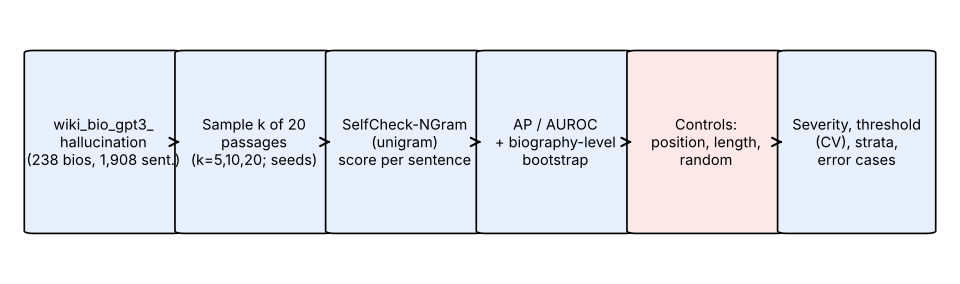
\includegraphics[width=\columnwidth]{fig6_pipeline.png}
\caption{Study pipeline. Red box: controls that use no sampled passages.}
\end{figure}

\section{Baseline Validation}
The detector is the official package, so validation targets the data and my evaluation code. Integrity checks (no missing values, label/binary consistency, identical sentence rows across $k$) pass. My re-implementation of the bootstrap reproduces all mean and CI values saved in the original Colab run to within $10^{-16}$. The random-score control gives AUROC 0.499 and AP 0.728, as expected. I have \emph{not} compared my numbers with those reported in the original SelfCheckGPT paper; protocol details (score variant, sample count, positive class) may differ, so the results here are not claimed to reproduce it \todo{TO VERIFY}.

\section{Results}
\subsection{Sample budget (RQ1)}
\begin{table}[t]\centering\small
\caption{Seed-42 point estimates and 95\% biography-level bootstrap CIs. Seed std is over seeds 42--46 (zero at $k=20$ by construction).}
\resizebox{\columnwidth}{!}{\begin{tabular}{lccc}\toprule
 & AUROC & 95\% CI & AP (95\% CI)\\\midrule
$k=5$ & 0.589 & 0.552--0.624 & 0.777 (0.739--0.815)\\
$k=10$ & 0.629 & 0.595--0.665 & 0.800 (0.763--0.835)\\
$k=20$ & 0.655 & 0.621--0.688 & 0.815 (0.780--0.849)\\\midrule
Position control & 0.582 & 0.555--0.611 & 0.774\\
Length control & 0.490 & 0.456--0.525 & 0.708\\
Random control & 0.499 & 0.469--0.528 & 0.728\\
Chance & 0.500 & -- & 0.730\\\bottomrule
\end{tabular}}\end{table}
AUROC and AP increase with $k$ (Fig.~\ref{fig:k}). The paired difference between $k=20$ and $k=5$ is $+0.066$ AUROC (CI 0.053--0.079) and $+0.038$ AP (CI 0.029--0.048). Across seeds, AUROC at $k=5$ is $0.5955\pm0.0045$ and at $k=10$ $0.6293\pm0.0022$ (std over 5 seeds), so subset choice matters far less than the sampling of biographies. Gains from 10 to 20 are smaller than from 5 to 10 (+0.025 vs.\ +0.040 AUROC, seed 42), but I did not test curvature or $k>20$.
\begin{figure}[t]\centering
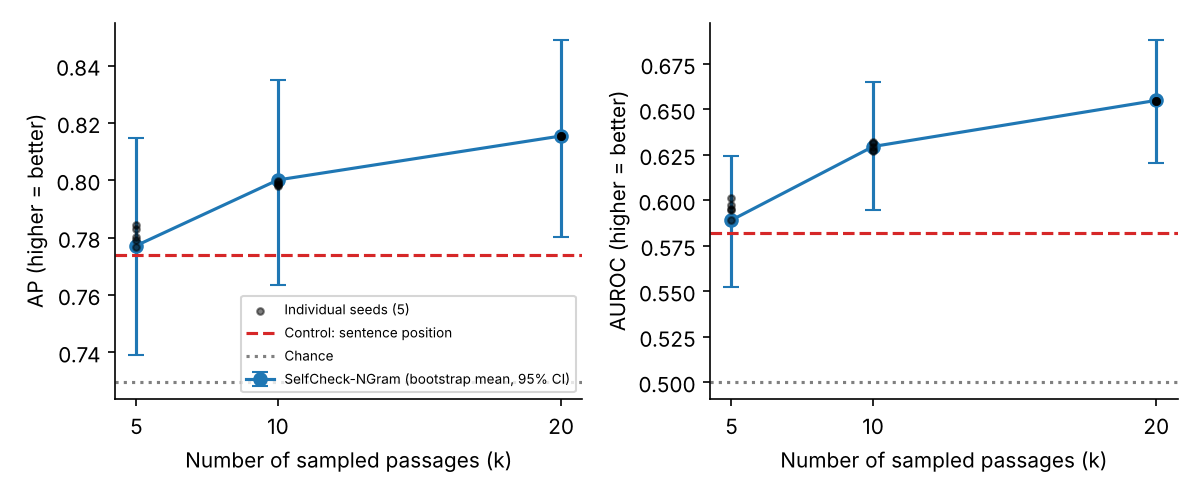
\includegraphics[width=\columnwidth]{fig1_metric_vs_k.png}
\caption{AP and AUROC vs.\ number of samples $k$: bootstrap mean with 95\% CI, individual seeds (black), position control (dashed red), chance (dotted).}\label{fig:k}
\end{figure}

\subsection{Comparison with controls (RQ2)}
\begin{table}[t]\centering\small
\caption{Paired AUROC differences (SelfCheck minus control), 95\% bootstrap CI.}
\begin{tabular}{lcc}\toprule
Comparison & Diff. & 95\% CI\\\midrule
$k=5$ vs.\ position & $+0.007$ & $-0.036$ to $0.047$\\
$k=10$ vs.\ position & $+0.048$ & $0.006$ to $0.087$\\
$k=20$ vs.\ position & $+0.073$ & $0.033$ to $0.115$\\
$k=20$ vs.\ length & $+0.165$ & $0.119$ to $0.214$\\\bottomrule
\end{tabular}\end{table}
The sentence-position control alone reaches AUROC 0.582 and AP 0.774 (later sentences are more often inaccurate). At $k=5$ SelfCheck-NGram cannot be distinguished from it; at $k=10$ the interval only just excludes zero; at $k=20$ the margin is modest ($+0.073$ AUROC, AP difference $+0.042$, CI 0.017--0.067). The length and random controls are at chance (Fig.~\ref{fig:ctl}).
\begin{figure}[t]\centering
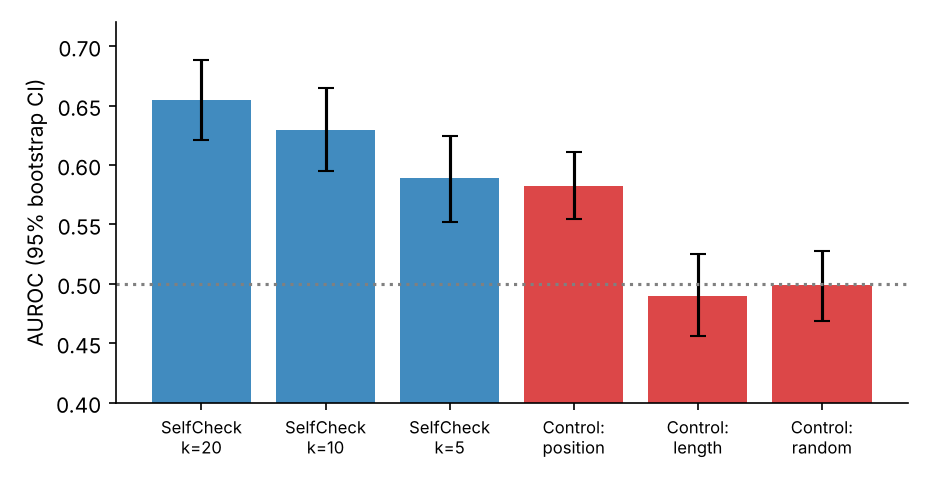
\includegraphics[width=0.85\columnwidth]{fig2_method_vs_controls.png}
\caption{AUROC with 95\% bootstrap CI: SelfCheck-NGram vs.\ controls.}\label{fig:ctl}
\end{figure}

\subsection{Severity and threshold (RQ3)}
At $k=20$ mean scores rise with severity: accurate 4.712, minor 4.844, major 4.988 (Fig.~\ref{fig:sev}). Major-vs-accurate AUROC is 0.696 (AP 0.744), minor-vs-accurate 0.605 (AP 0.619), and major-vs-minor 0.608, so major inaccuracies are separated more easily than minor ones.

\begin{table}[t]\centering\small
\caption{Threshold at $k=20$ (Youden's $J$). Flag rates are the fraction of sentences predicted inaccurate.}
\resizebox{\columnwidth}{!}{\begin{tabular}{lcc}\toprule
 & In-sample & 5-fold grouped CV\\\midrule
Threshold & 4.648 & 4.632--4.705\\
Accuracy & 0.692 & 0.680\\
Precision / recall (inaccurate) & 0.805 / 0.763 & 0.800 / 0.749\\
Flagged: major / minor & 0.821 / 0.693 & 0.808 / 0.677\\
Flagged: accurate (false alarms) & 0.500 & 0.506\\\bottomrule
\end{tabular}}\end{table}
Choosing the threshold on the evaluation data inflates accuracy by about 0.012, so the effect is small here. A more important observation is that the best single threshold flags about half of the accurate sentences, which would make the detector hard to use for abstention without further filtering.
\begin{figure}[t]\centering
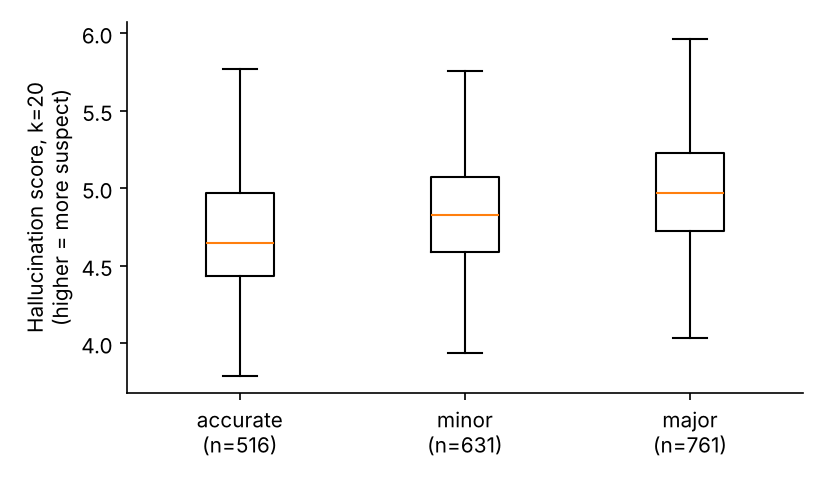
\includegraphics[width=0.85\columnwidth]{fig3_score_by_label.png}
\caption{Score distribution by human label ($k=20$, outliers hidden).}\label{fig:sev}
\end{figure}


\begin{figure}[t]\centering
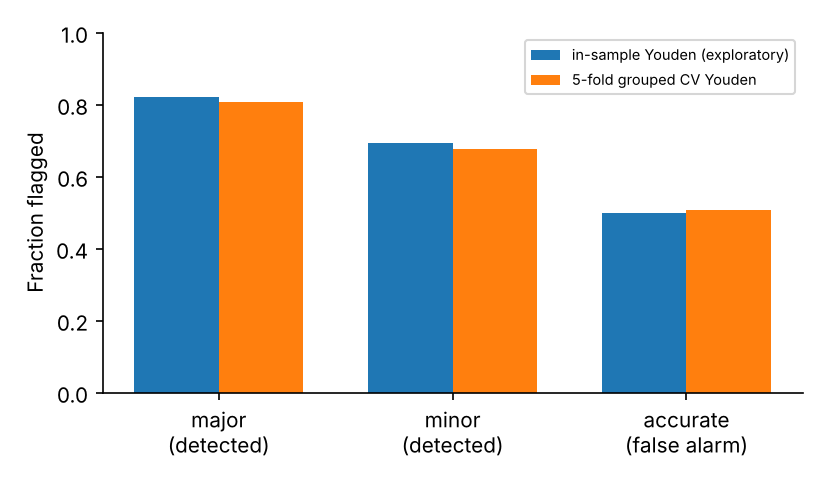
\includegraphics[width=0.85\columnwidth]{fig5_detection_by_severity.png}
\caption{Fraction of sentences flagged, by human label, for the in-sample and grouped-CV thresholds ($k=20$).}\label{fig:det}
\end{figure}

\subsection{Error cases}
I inspected the 25 highest-scoring accurate sentences (false positives) and the 25 lowest-scoring inaccurate sentences (false negatives) under the grouped-CV threshold (\texttt{results/tables/false\_*\_top25.csv}). This is a qualitative look at extreme cases, not a representative sample. The false positives are mostly vague or generic statements about a person's career or character (for example, a sentence about ``later years marred by personal problems'', or about influencing ``various generations'' of artists); the mean position of these cases is 5.3, later than typical. The false negatives are mostly specific claims (dates, places, offices, medals) that humans marked wrong but that score low; their mean position is 4.0 (median 2), they are shorter than the false positives (mean 81 vs.\ 103 characters), and a few are sentences truncated in the dataset itself (for instance ending in ``and'' or ``to the''). A plausible reading is that the samples repeat the same specific but wrong details, so a consistency check under-flags them, while generic statements contain words that rarely occur in the samples; I did not test this explanation.

\subsection{Position strata}
AUROC at $k=20$ differs by sentence position: 0.739 for positions 0--1 (n=476), 0.643 for positions 2--4 (n=706) and 0.566 for position 5 or later (n=726) (Fig.~\ref{fig:pos}). Prevalence also rises with position (0.647, 0.725, 0.788).
\begin{figure}[t]\centering
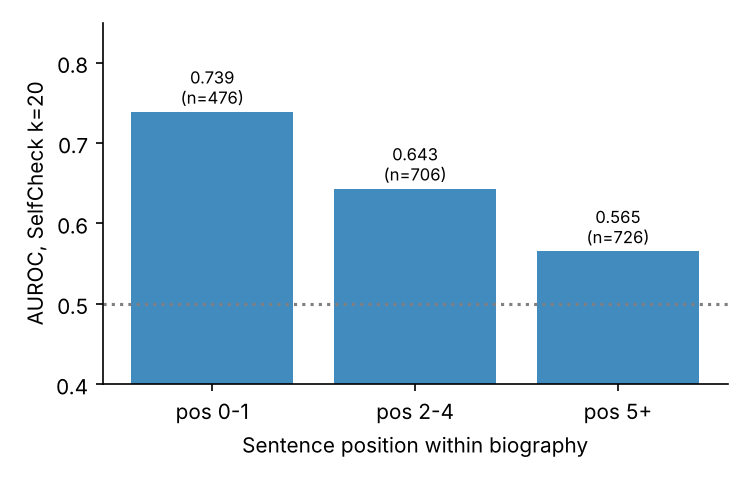
\includegraphics[width=0.8\columnwidth]{fig4_auroc_by_position.png}
\caption{SelfCheck-NGram AUROC ($k=20$) by sentence position.}\label{fig:pos}
\end{figure}

\section{Discussion}
\textbf{Direct observations.} More samples help; the detector beats chance at all $k$; it is statistically tied with a position heuristic at $k=5$ and ahead of it by a small margin at $k=20$; major errors are easier than minor ones; its separation is much weaker later in a biography.

\textbf{Possible explanations (untested).} A unigram model compares word frequencies, so it may be most informative when early sentences state facts (names, dates, places) that the samples either repeat or contradict, and less informative later where generic words may dominate. The position effect on prevalence and the position effect on AUROC may be related, but this study cannot separate them.

\textbf{Alternative explanation for the AP value.} AP of 0.815 looks strong but the chance level is 0.730; AUROC (0.655) is the more informative summary here.

\textbf{Unsupported claims.} I do not claim that the results transfer to other generators, domains, or to stronger SelfCheckGPT variants (which I did not run), nor that gains continue for $k>20$.

\textbf{Follow-ups ranked by cost and expected information.} (1) Run one stronger published variant under the same protocol (about 20 minutes per variant in Colab). (2) Fit a position-adjusted detector or report within-position AUROC to separate the confounds. (3) Repeat on a second dataset or generator.

\section{Limitations}
One dataset and one generator (GPT-3 biographies); one unigram detector; no second published method; positive class is the majority (73\%); one annotation set with no inter-annotator information used; the protocol was fixed retrospectively; the 5-seed spread only varies subsets at $k=5,10$; no comparison with the original paper's reported numbers; library versions used in Colab were not recorded; the threshold CV uses a single partition; sentence length was measured in characters only.

\section{Conclusion}
On this benchmark, a unigram SelfCheck detector improves steadily with the number of sampled passages and is tied with a sentence-position heuristic at $k=5$, marginally ahead at $k=10$, and ahead by a modest margin at $k=20$. Reported AP overstates its usefulness because of class imbalance, and a single threshold flags half of the accurate sentences. These conclusions concern one detector variant on one dataset and should not be generalized without further experiments.

\section*{AI Assistance Disclosure}
AI assistance (Claude, Anthropic) was used for code generation, debugging suggestions, analysis scripts, figure generation and drafting of this manuscript, under the student's instruction; the student's Colab notebook produced the raw scores. A detailed record, including two real tool errors and one methodological issue caught during the work, is in \texttt{ai\_assistance\_log.md}. The bibliography was written from the assistant's memory and must be checked against the original sources.

\section*{Reproducibility}
Repository: \todo{GitHub URL}. Environment, seeds and commands are in the README. \texttt{python scripts/evaluate.py} and \texttt{python scripts/make\_figures.py} regenerate every table and figure from \texttt{results/raw/} (executed; Python 3.12.3). Regenerating the raw scores (\texttt{scripts/run\_selfcheck.py}, about 20 minutes per seed in Colab) is \todo{TEST REQUIRED} as a standalone script.

\bibliographystyle{plain}
\bibliography{references}
\end{document}
